\documentclass[UTF8, 16pt]{beamer}
 
% Chinese
\usepackage{xeCJK}

% Font
\usepackage{bookman}
\usefonttheme{serif}
% \usepackage[T1]{fontenc}
%\usepackage{tgbonum}

% Other packages
\usepackage{hyperref}
\usepackage{appendixnumberbeamer}
\usepackage{latexsym}
\usepackage{amsmath}
\usepackage{xcolor}
\usepackage{multicol}
\usepackage{booktabs}
\usepackage{graphicx}
\usepackage{listings}
\usepackage{stackengine}

% SUFE.sty
\usepackage{SUFE} 
% Bibtex
\usepackage[citestyle=authoryear-comp, 
            backend=biber, 
            bibstyle=numeric, 
%			sorting=ynt
            ]{biblatex}
\setbeamertemplate{bibliography item}[text]
\addbibresource{ref.bib}

% Other setting
\setlength{\parskip}{1em} % 设置段落之间的间距为 1em
\graphicspath{{res/}}
\setCJKmainfont{PingFang SC}
\setCJKmonofont{Yahei Mono}

%%%%%%%%%%%%%%%%%%%%%%%%%%

% Title page
%% Author
\author[计算机协会] % The short name
{
%Name
计算机协会
%\inst{1}
%\and
%XXX 
%\inst{2}
} 
%% Title & Subtitle
\title[Command-Line 命令行教学]{Command-Line 命令行教学}
\subtitle{缺失的一课}
%% Institution
\institute[SUFE]
{
%\inst{1}
% Shanghai University of Finance and Economics
上海财经大学
%\and
%\inst{2}
%Shanghai University of Finance and Economics
}
%% Date
\date{23会计学院\ ACCA\ 张华轩}
%%Logo
%\logo{
\includegraphics[height=1cm]{sufe_logo}}

%%%%%%%%%%%%%%%%%%%%%%%%%%

% Document begins
\begin{document}

%Title page
\begin{frame}[noframenumbering]
    %	\thispagestyle{empty}
    \titlepage{}
    % Logo
    \vspace{-0.5cm}
    \begin{figure}[htpb]
        \begin{center}
            
\includegraphics[width=0.19 \linewidth]{sufe_logo.png}
            \quad
            
\includegraphics[width=0.19 \linewidth]{ca_logo.png}
        \end{center}
    \end{figure}
\end{frame}

% % Contents page
% \begin{frame}{Contents}
% 	\tableofcontents[sectionstyle=show,
% 		subsectionstyle=show/shaded/hide,
% 		subsubsectionstyle=show/shaded/hide]
% \end{frame}

% Body
\section{前言}
\begin{frame}
    \textcolor{sufered}{
        操作系统 \quad
        计算机网络 \quad
        计算机硬件 \quad
        数据库 \quad
        编译原理 \\
        数据结构与算法 \quad
        程序设计 \quad
        软件工程 \quad
        编程语言 \quad
        \dots\dots
    }
\end{frame}

\begin{frame}
    \textcolor{sufered}{
        操作系统 \quad
        计算机网络 \quad
        计算机硬件 \quad
        数据库 \quad
        编译原理 \\
        数据结构与算法 \quad
        程序设计 \quad
        软件工程 \quad
        编程语言 \quad
        \dots\dots
    }

    都不是今天要学的东西\dots\dots
\end{frame}

\begin{frame}
    \centering
    \textcolor{sufered}{Vim 文本编辑}
    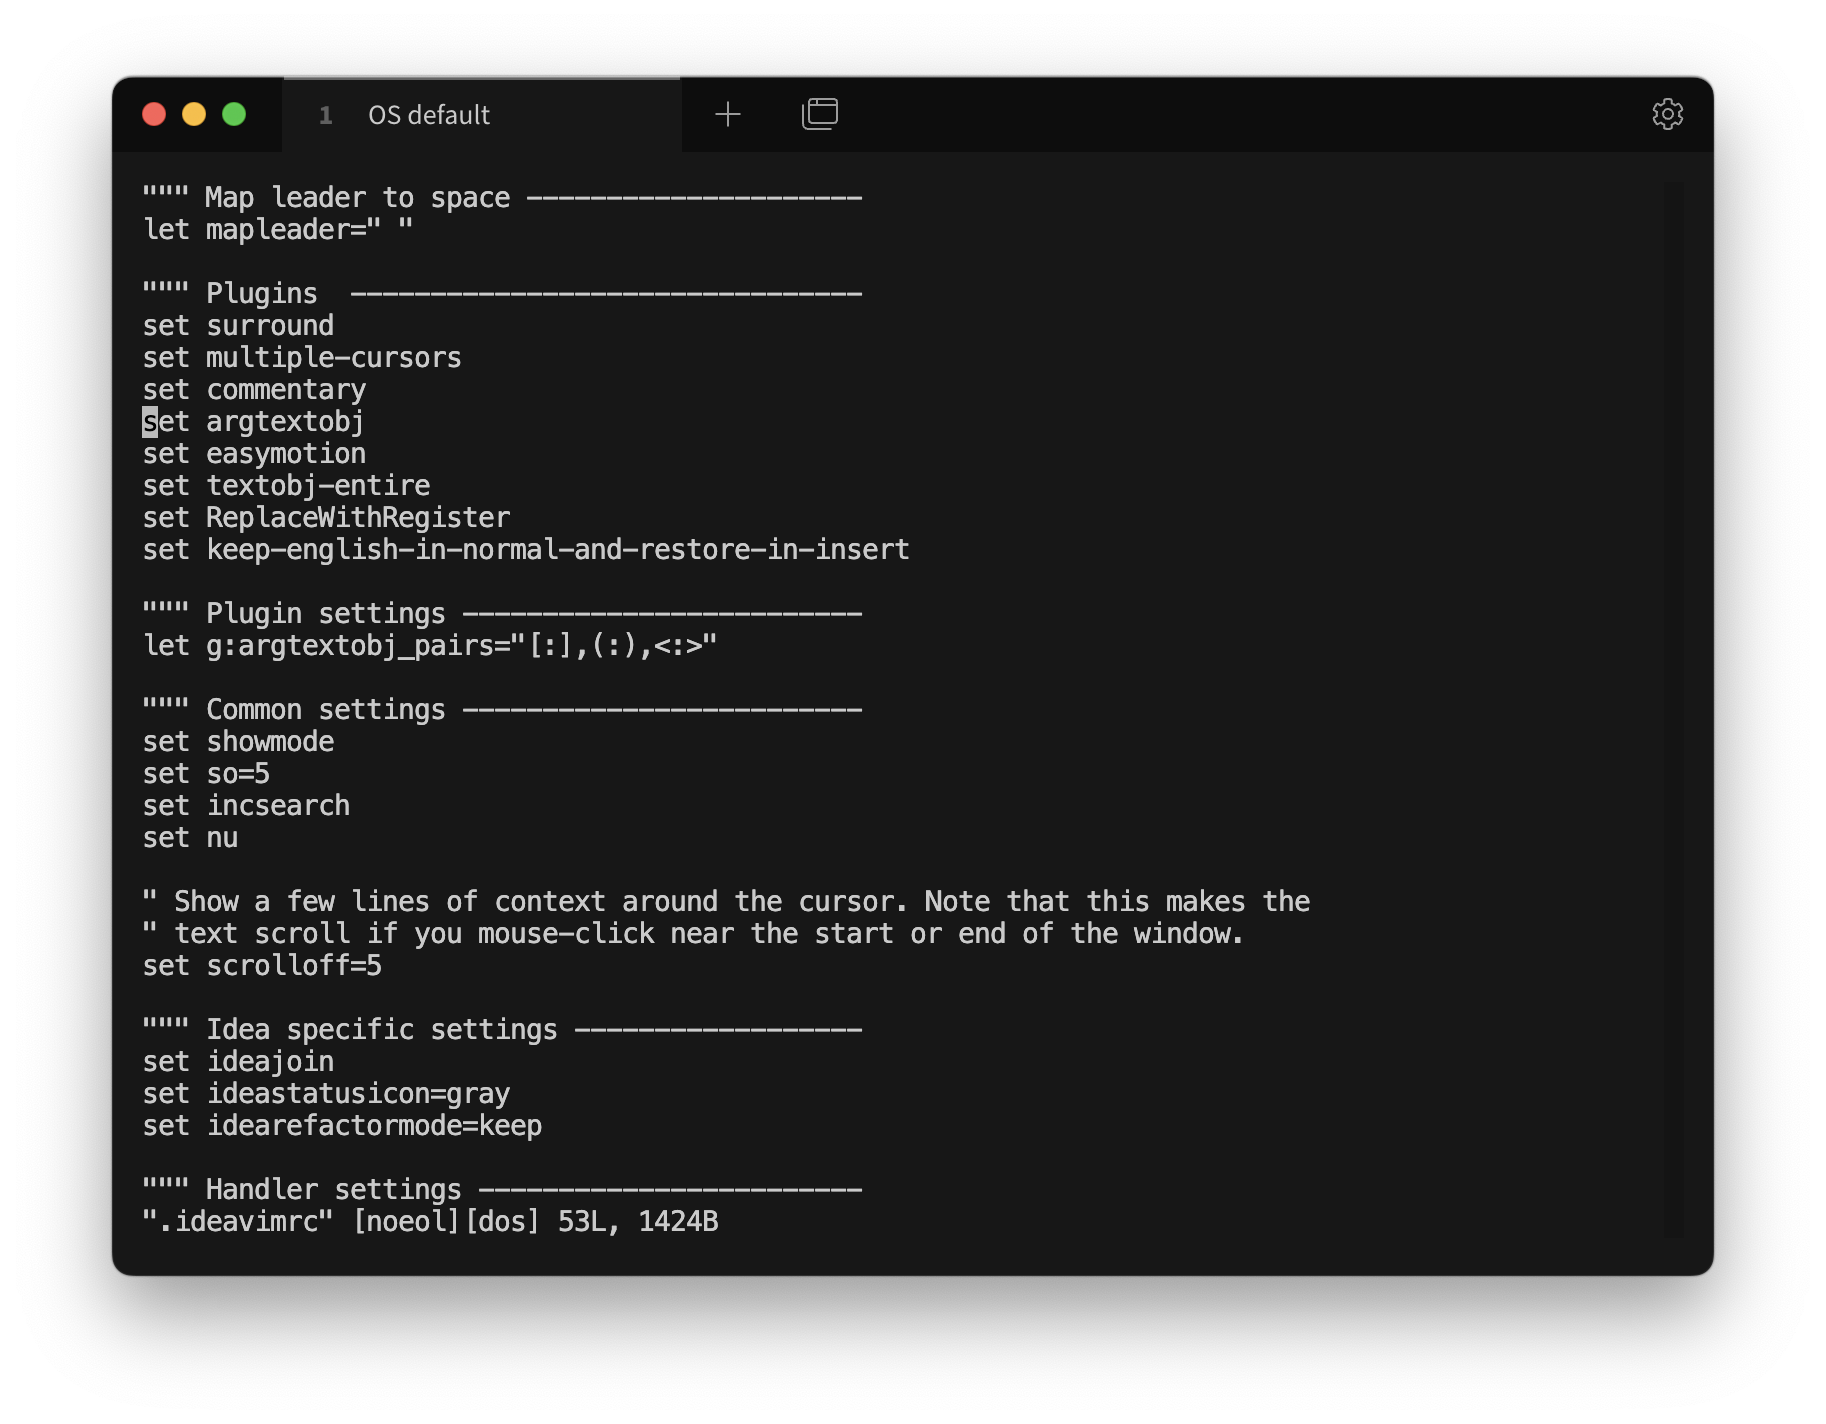
\includegraphics[width=0.95\linewidth]{vim.png}
\end{frame}

\begin{frame}
    \centering
    \textcolor{sufered}{Find 查找文件}
    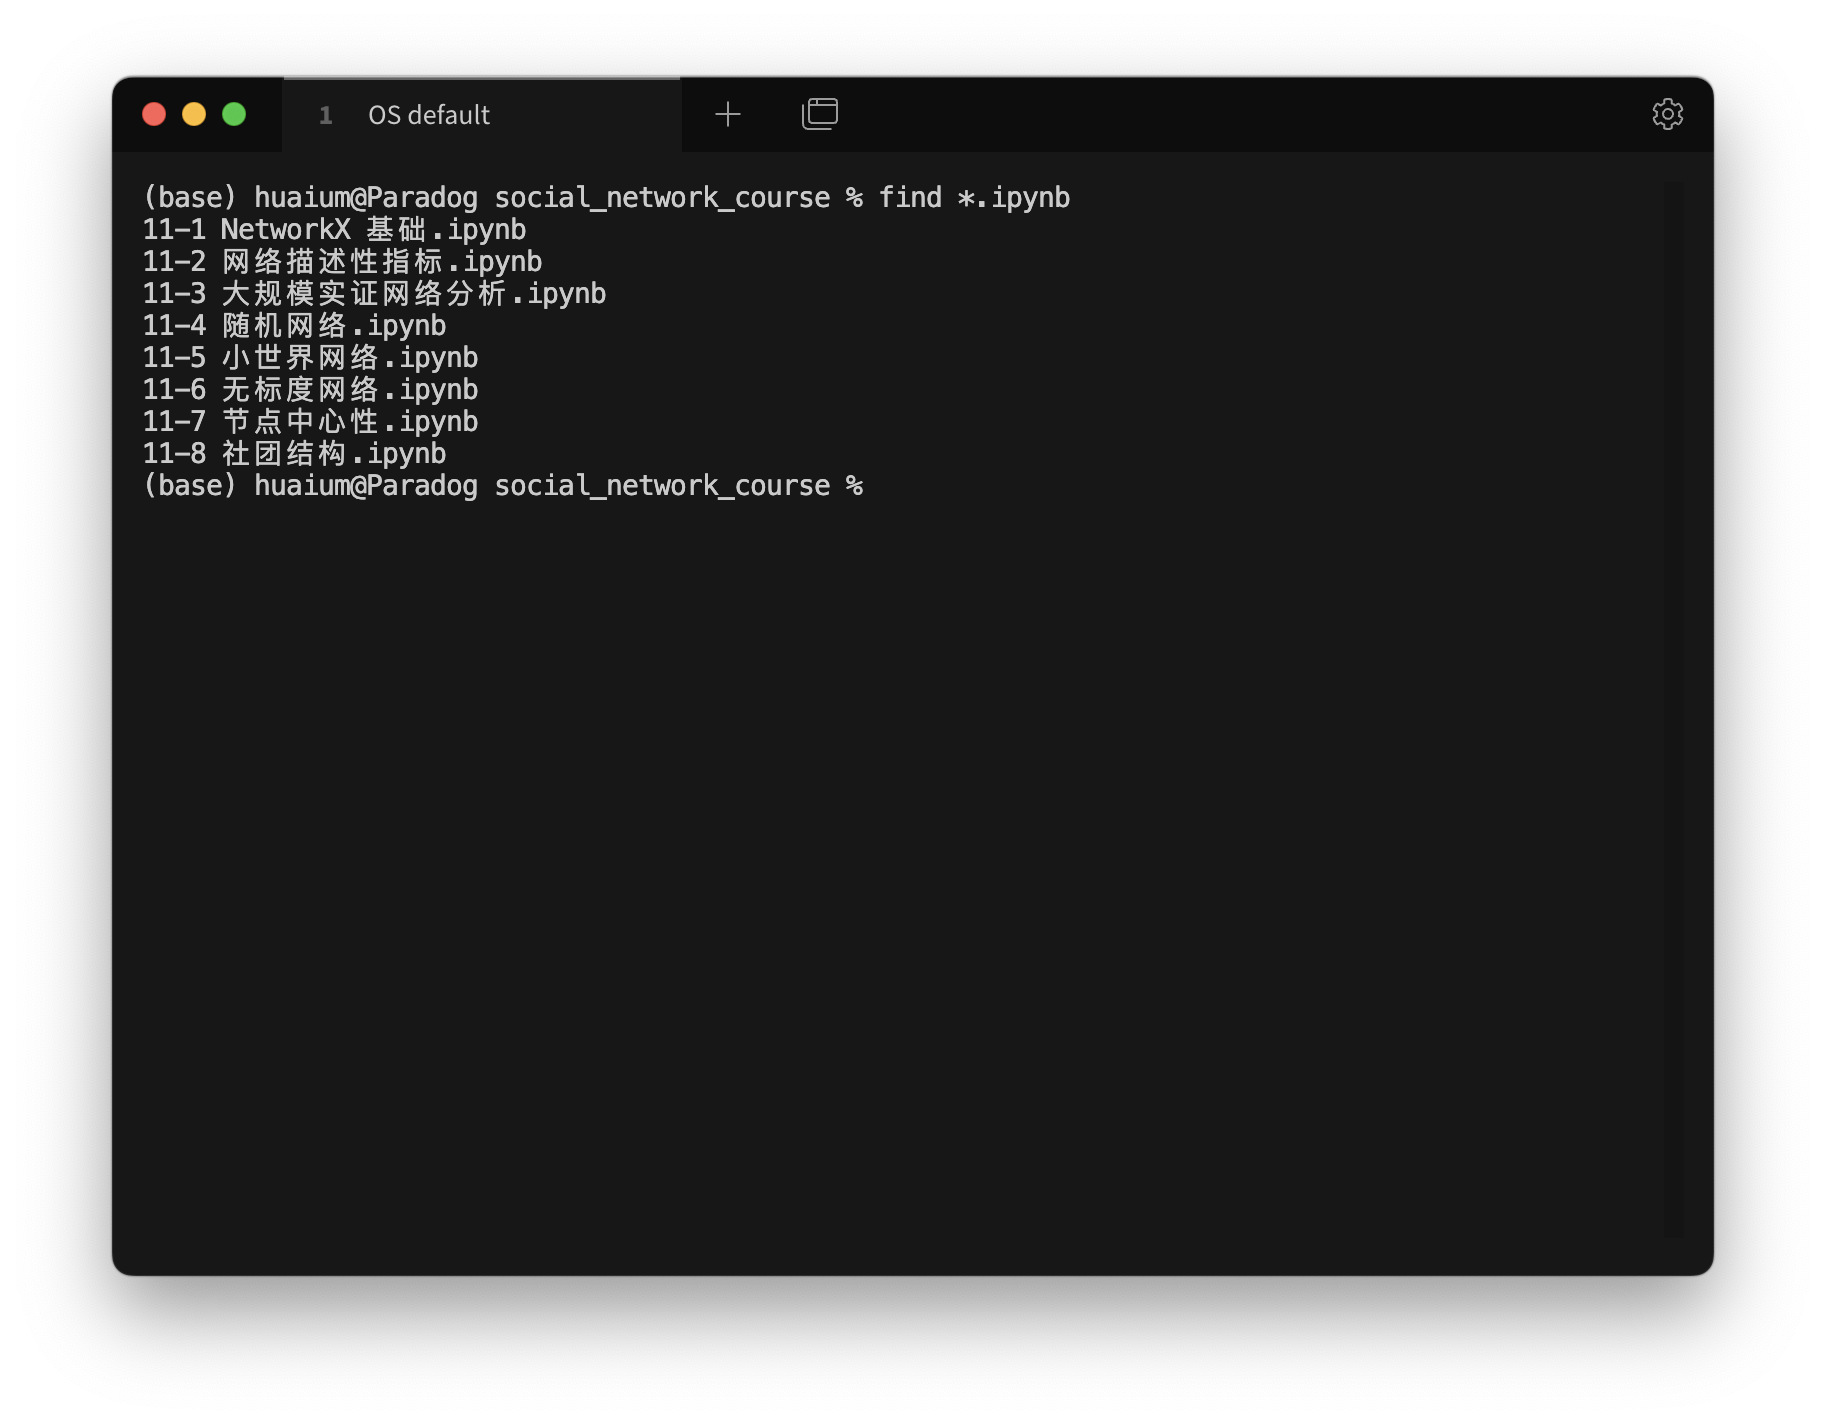
\includegraphics[width=0.95\linewidth]{find.png}
\end{frame}

\begin{frame}
    \centering
    \textcolor{sufered}{SSH 远程主机}
    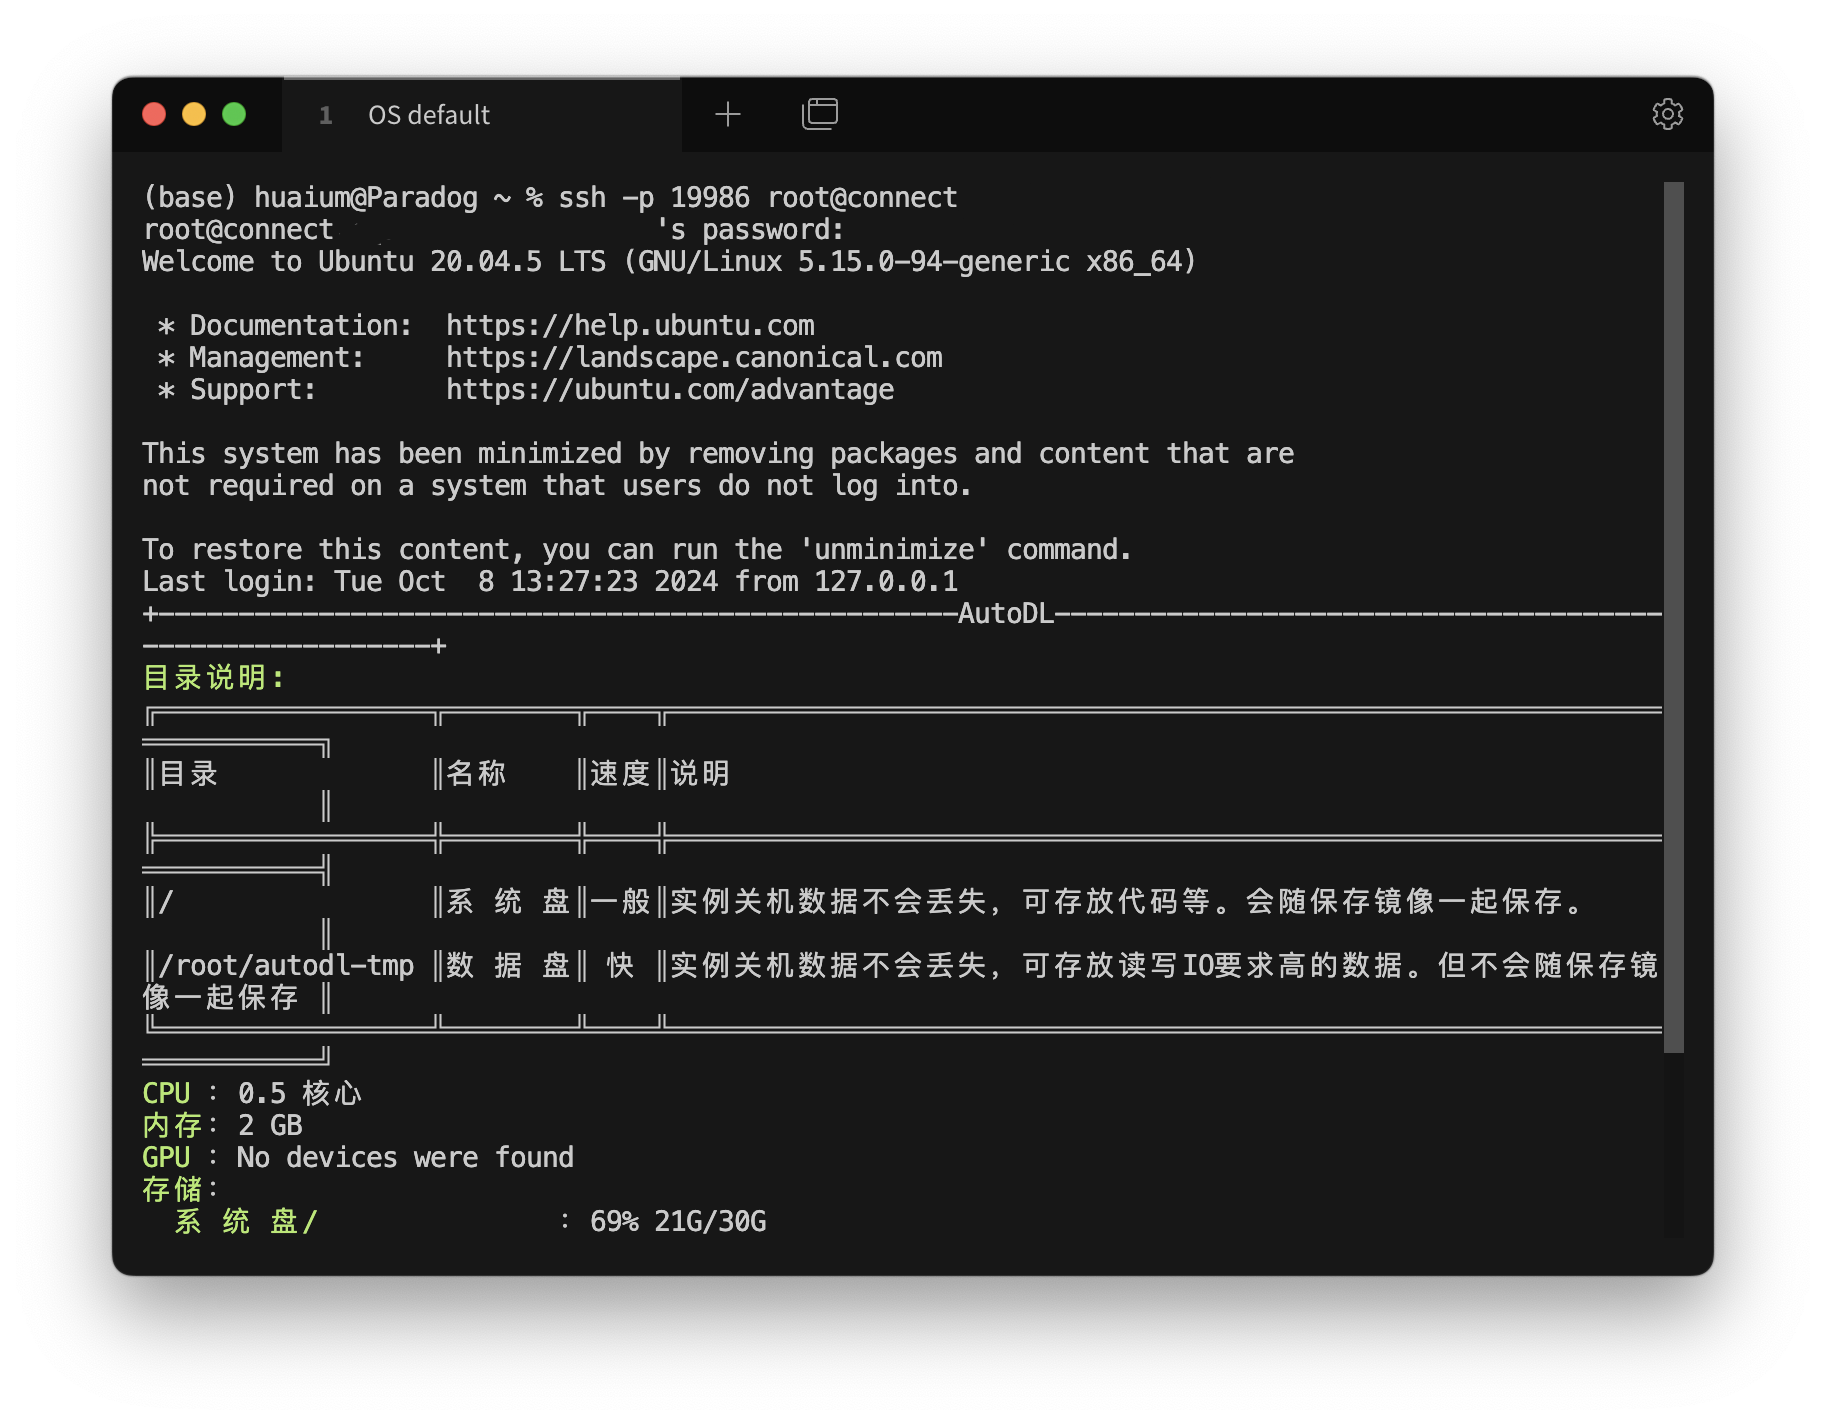
\includegraphics[width=0.95\linewidth]{ssh.png}
\end{frame}

\section{Shell 命令行}

\begin{frame}
    \frametitle{什么是 Shell}
    \begin{itemize}
        \item Shell 是用户与操作系统内核之间的接口,通过 Shell 可以运行命令、启动程序、管理文件系统等
        \item Shell 既可以作为交互式解释器(处理用户输入的命令),也可以用于执行脚本文件(自动化任务)
        \item 常见的 Shell 类型:
              \begin{itemize}
                  \item Bourne Shell (\texttt{sh})
                  \item Bourne Again Shell (\texttt{bash})
                  \item Z Shell (\texttt{zsh})
                  \item C Shell (\texttt{csh})
              \end{itemize}
        \item Shell 有时和“终端”混用,但实际有区别
    \end{itemize}
\end{frame}

\begin{frame}[fragile]
    \frametitle{不同平台下的 Shell}
    \begin{alertblock}{Linux}
        \begin{itemize}
            \item 最常用的 Shell 是 \texttt{bash},默认安装在大多数 Linux 发行版中
            \item 其他 Shell 包括 \texttt{zsh} 和 \texttt{fish}
        \end{itemize}
        \begin{lstlisting}[language=bash]
pwd # 显示当前目录
ls -l # 列出文件
        \end{lstlisting}
    \end{alertblock}
\end{frame}

\begin{frame}[fragile]
    \frametitle{不同平台下的 Shell}
    \begin{alertblock}{Windows}
        \begin{itemize}
            \item 传统命令行工具是 \texttt{cmd},现代 Windows 推荐使用 \texttt{PowerShell} 和 \texttt{Windows Terminal}
            \item Windows 10 及以上版本支持 \texttt{WSL} (Windows Subsystem for Linux),可以运行 Linux 命令
        \end{itemize}
        \begin{lstlisting}[language=bash]
# 在 PowerShell 中列出文件
Get-ChildItem
        \end{lstlisting}
    \end{alertblock}
\end{frame}

\begin{frame}[fragile]
    \frametitle{不同平台下的 Shell}
    \begin{alertblock}{macOS}
        \begin{itemize}
            \item macOS 基于 Unix,默认使用 \texttt{zsh},之前的版本使用 \texttt{bash}
            \item 支持大多数 Unix/Linux 命令,可以通过 \texttt{Homebrew} 安装额外工具
        \end{itemize}
        \begin{lstlisting}[language=bash]
# 安装软件包
brew install wget
        \end{lstlisting}
    \end{alertblock}
\end{frame}

\begin{frame}
    \frametitle{环境配置}
    \textcolor{sufered}{基于类 Unix 命令行进行讲解}

    \begin{itemize}
        \item \texttt{Linux 和 macOS}:均为类 Unix 系统,支持 POSIX 规范的命令行
        \item \texttt{Windows}:需要安装 MSYS2 开发环境
    \end{itemize}
    \url{https://www.msys2.org}
\end{frame}

\begin{frame}
    \frametitle{单个命令}
    \textcolor{sufered}{最简单的结构,仅由一个命令组成}

    \begin{itemize}
        \item \texttt{ls (list)}
        \item \texttt{pwd (print working directory)}
        \item \texttt{whoami (Who am I?)}
    \end{itemize}
    可以直接运行,不需要额外参数
\end{frame}

\begin{frame}[fragile]
    \frametitle{参数对象命令}
    \textcolor{sufered}{命令 + [参数] + [操作对象] + [\dots] (方括号表示可选)}

    参数用于改变命令的行为,通常以短格式(如 \texttt{-l})或长格式(如 \texttt{--long})表示
    \begin{lstlisting}[numbers=none]
ls -l\end{lstlisting}
    \begin{lstlisting}[numbers=none]
grep --ignore-case "error" fake.log\end{lstlisting}
    \begin{lstlisting}[numbers=none]
cp file1.txt file2.txt\end{lstlisting}
\end{frame}

\begin{frame}[fragile]
    很多短格式参数是长格式参数的缩写,等价于后者
    \begin{lstlisting}
ls -l
ls -list # 等价长格式参数\end{lstlisting}
    \begin{lstlisting}
grep --ignore-case "error" fake.log
grep -i "error" fake.log # 等价短格式参数\end{lstlisting}
\end{frame}

\begin{frame}
    \frametitle{类 Unix 文件权限系统}

    在类 Unix 系统(笼统来说就是 Unix 和 Linux)中,每个文件和目录都有一组权限,决定用户对文件或目录的操作方式。权限分为三类:
    \begin{itemize}
        \item \textbf{所有者}(User):文件或目录的拥有者
        \item \textbf{群组}(Group):与文件所有者同属一个群组的用户
        \item \textbf{其他人}(Other):所有其他用户
    \end{itemize}
\end{frame}

\begin{frame}
    \centering
    \textcolor{sufered}{类 Unix 用户和用户组}
    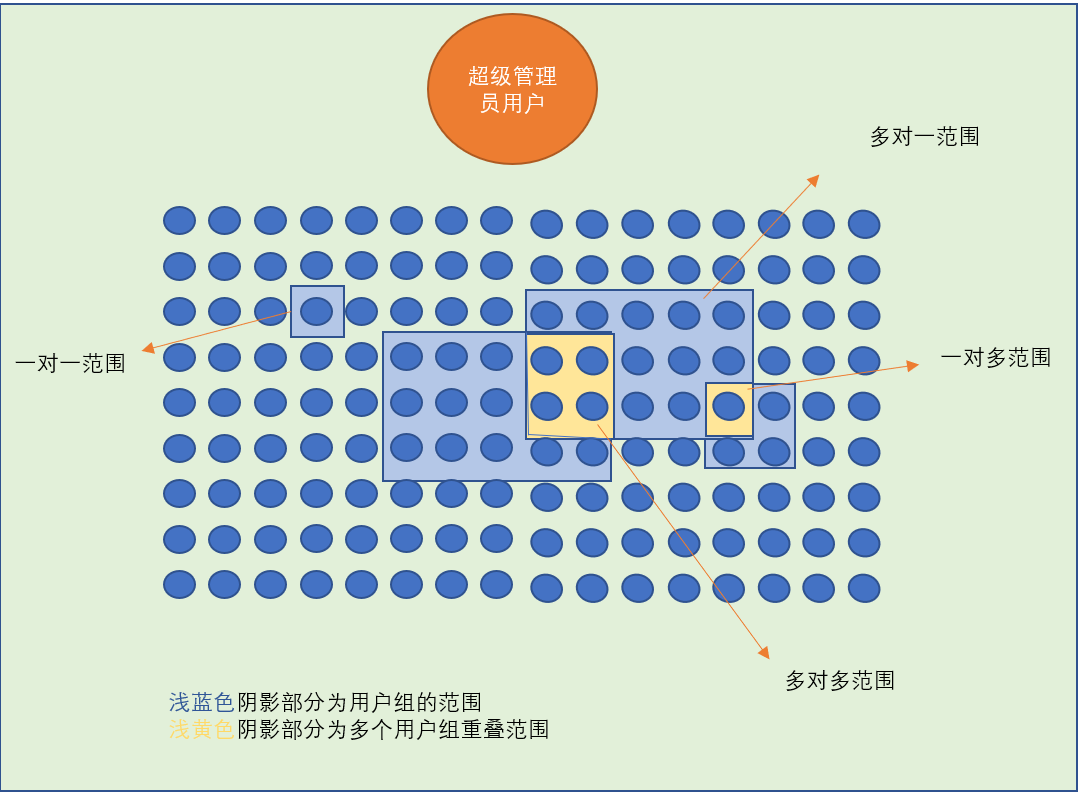
\includegraphics[width=0.95\linewidth]{shell/user.png}
\end{frame}

\begin{frame}
    \frametitle{文件类型}
    \textcolor{sufered}{共七类,其中最常见的三类为:}

    \begin{itemize}
        \item \textbf{普通文件}(regular file)用 \texttt{-} 表示
        \item \textbf{目录}(directory)用 \texttt{d} 表示
        \item \textbf{符号链接}(symlink, symbolic link)用 \texttt{l} 表示
    \end{itemize}

    此外还有块设备(\texttt{b} 驱动器)、字符设备(\text{c} 输入输出设备)、命名管道(\texttt{p} 进程单向通信)和套接字(\texttt{s} 网络通信)
\end{frame}

\begin{frame}
    \frametitle{权限符号解释}

    权限由十个字符表示,例如:\texttt{-rw-r--r--}。第一个字符表示文件类型,其后的九个字符分为三组,依次为:
    \begin{itemize}
        \item \texttt{r}:读权限(read)
        \item \texttt{w}:写权限(write)
        \item \texttt{x}:执行权限(execute)
    \end{itemize}
    三组分别代表\textbf{所有者}、\textbf{群组}、\textbf{其他人}的权限
\end{frame}

\begin{frame}
    \frametitle{Example}
    \textcolor{sufered}{\texttt{-rw-r--r--} 的含义如下:}

    \begin{itemize}
        \item \texttt{-}:文件类型(- 表示普通文件,d 表示目录)
        \item \texttt{rw-}:所有者有读写权限,但没有执行权限
        \item \texttt{r--}:群组只有读权限
        \item \texttt{r--}:其他人也只有读权限
    \end{itemize}
    可以通过 \texttt{chmod} 命令进行修改
\end{frame}

\begin{frame}[fragile]
    \frametitle{常用权限命令}

    \begin{itemize}
        \item \texttt{ls -l}:列出文件的详细信息,包括权限
        \item \texttt{chmod}:改变文件或目录的权限
        \item \texttt{chown}:改变文件的所有者和群组
    \end{itemize}
    \begin{lstlisting}
chmod u+x filename # 为文件所有者添加执行权限
chmod g-w filename # 为文件删除群组写权限
chmod a+x filename # 为所有用户添加执行权限
chmod u=rw,go=r filename # 将所有者的权限设置为读、写,组和其他用户的权限设置为只读\end{lstlisting}
\end{frame}

\begin{frame}[fragile]
    \frametitle{八进制权限}
    \textcolor{sufered}{每个权限都对应一个数值:}

    \begin{itemize}
        \item 4:读 r,即 $2^2$
        \item 2:写 w,即 $2^1$
        \item 1:执行 x,即 $2^0$
    \end{itemize}
    \begin{lstlisting}[numbers=none]
chmod 755 filename # 代表什么?\end{lstlisting}
\end{frame}

\begin{frame}[fragile]
    \frametitle{管道命令}

    使用管道符 \texttt{|} 将一个命令的输出作为下一个命令的输入
    \begin{lstlisting}
cat file.txt | grep "pattern"
cat file.txt | grep "pattern" | head -n 10\end{lstlisting}
    管道命令用于将多个命令组合在一起,形成复杂操作
\end{frame}

\begin{frame}
    \centering
    \textcolor{sufered}{管道命令}

    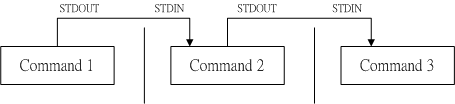
\includegraphics[width=0.95\linewidth]{shell/pipe.png}
\end{frame}

\begin{frame}[fragile]
    \frametitle{后台执行命令}

    在命令后加上 \texttt{\&},可以将命令放到后台执行
    \begin{lstlisting}[numbers=none]
ping -c 4 google.com &\end{lstlisting}
    \begin{lstlisting}[numbers=none]
sleep 8 &\end{lstlisting}
    后台执行允许命令运行时继续进行其他操作
\end{frame}

\begin{frame}[fragile]
    \frametitle{重定向命令}

    重定向命令将命令的输出重定向到文件,或者将文件作为命令的输入
    \begin{lstlisting}
echo "Hello" > output.txt  # 输出重定向
sort < input.txt           # 输入重定向\end{lstlisting}
    \texttt{>} 覆盖写入文件,\texttt{>>} 追加写入文件

    有没有 \texttt{<<} ?
\end{frame}

\begin{frame}[fragile]
    \frametitle{文件结束符 EOF}

    EOF(End Of File)在计算机中是表示文件或数据流结束的标志

    在不同数据流中,EOF 的含义和处理略有不同
    \begin{itemize}
        \item \texttt{文件操作:EOF 标志表示文件的结束}
        \item \texttt{命令行输入:Ctrl+D or Ctrl+Z}
    \end{itemize}
    \begin{lstlisting}
cat << EOF
This is a line of text.
This is another line of text.
EOF\end{lstlisting}
    此处的 EOF 可以用其他字符代替
\end{frame}

\begin{frame}[fragile]
    \frametitle{复杂重定向}
    \textcolor{sufered}{假设 \texttt{nonexistent\_dir} 不存在:}

    \begin{lstlisting}[numbers=none]
{ ls -l /nonexistent_dir 2>&1 && echo "Directory listed successfully" ; } >output.log 2>error.log\end{lstlisting}

    ???
\end{frame}

\begin{frame}[fragile]
    \frametitle{标准输入输出}

    在命令行环境中,通常有三种标准输入输出流,它们通过文件描述符来表示:

    \begin{itemize}
        \item \textbf{标准输入 (stdin)}: 对应文件描述符 \texttt{0},用于接收来自键盘或其他输入设备的数据
        \item \textbf{标准输出 (stdout)}: 对应文件描述符 \texttt{1},用于输出正常的命令结果,默认显示在终端中
        \item \textbf{标准错误 (stderr)}: 对应文件描述符 \texttt{2},用于输出错误消息,也显示在终端中,但与标准输出分开
    \end{itemize}

    \begin{lstlisting}[numbers=none]
command > output.txt 2> error.txt < input.txt\end{lstlisting}
    \begin{itemize}
        \item \texttt{> output.txt} 将标准输出重定向到 \texttt{output.txt} 文件
        \item \texttt{2> error.txt} 将标准错误输出重定向到 \texttt{error.txt} 文件
        \item \texttt{< input.txt} 将标准输入从 \texttt{input.txt} 文件中读取数据
    \end{itemize}
\end{frame}

\begin{frame}[fragile]
    \frametitle{逻辑运算法 \texttt{\&\&} 和 \texttt{||}}

    \begin{itemize}
        \item \texttt{\&\&}:逻辑与 (AND),表示前一个命令成功时才执行下一个命令。
        \item \texttt{||}:逻辑或 (OR),表示前一个命令失败时才执行下一个命令
    \end{itemize}

    \begin{lstlisting}
# 只有当第一个命令成功时,才会执行第二个命令
command1 && command2

# 如果第一个命令失败,则执行第二个命令
command1 || command2\end{lstlisting}
    \&\& 和 || 均采用断路判断
\end{frame}

\begin{frame}[fragile]
    \frametitle{其他逻辑运算符}

    \begin{itemize}
        \item \texttt{;}:无论前一个命令是否成功,都会执行后续命令
        \item \texttt{!}:逻辑非,反转命令的退出状态
        \item \texttt{()}:在子 shell 中执行一组命令
        \item \texttt{\{\}}:在当前 shell 中执行一组命令
    \end{itemize}

    \begin{lstlisting}
# command1 和 command2 无论成功与否都会依次执行
command1; command2

# 如果 command 失败,则返回成功的退出状态;反之亦然
! command

# 在子 shell 中执行 command1 和 command2
(command1 && command2)

# 在当前 shell 中执行 command1 和 command2
{ command1; command2; }\end{lstlisting}
\end{frame}

\begin{frame}[fragile]
    \frametitle{注意!!!}
    \textcolor{sufered}{区分 \texttt{\&} 和 \text{\&\&};\texttt{|} 和 \texttt{||}}

    \begin{lstlisting}
# command1 后台运行,command 2 前台执行
command1 & command2\end{lstlisting}
    \begin{lstlisting}
# 管道操作:将 command1 的输出作为 command2 的输入
command1 | command2\end{lstlisting}
\end{frame}

\begin{frame}[fragile]
    \frametitle{回过头来}
    \textcolor{sufered}{假设 \texttt{nonexistent\_dir} 不存在:}

    \begin{lstlisting}[numbers=none]
{ ls -l /nonexistent_dir 2>&1 && echo "Directory listed successfully" ; } >output.log 2>error.log\end{lstlisting}

    !!!
\end{frame}

\begin{frame}[fragile]
    \frametitle{SSH 远程主机}
    \textcolor{sufered}{SSH 连接的基本命令}

    \begin{lstlisting}
# 通过 SSH 连接到远程主机
ssh username@remote_host

# 连接时指定自定义端口
ssh -p 2222 username@remote_host

# 使用指定的私钥文件连接 (i->identity)
ssh -i /path/to/private_key username@remote_host
    \end{lstlisting}
\end{frame}

\begin{frame}[fragile]
    \frametitle{端口转发}
    \textcolor{sufered}{本地转发(local forwarding)}
    \begin{itemize}
        \item 创建一个本地端口,将发往该端口的所有通信都通过 SSH 服务器,转发到指定的远程服务器的端口
        \item -C:启用数据压缩
        \item -N:不执行远程命令,仅创建隧道,不打开远程 shell
        \item -g:允许远程主机连接到本地转发的端口
        \item -L lPort:127.0.0.1:rPort:设置本地端口转发,将本地 lPort 端口映射到远程服务器上的 rPort 端口
    \end{itemize}

    \begin{lstlisting}
# 连接时指定自定义端口
ssh -CNg -L lPort:127.0.0.1:rPort user@remote -p sPort
    \end{lstlisting}
\end{frame}

\begin{frame}[fragile]
    \frametitle{为什么要这样干?}

    \textcolor{sufered}{POSIX 可移植操作系统接口}

    \begin{itemize}
        \item \texttt{Portable Operating System Interface of UNIX}
        \item 1974年,贝尔实验室正式对外发布 \texttt{Unix}
        \item \texttt{Unix-like OS}: BSD, Sun Solaris
        \item 20世纪80年代中期,\texttt{Unix} 厂商试图通过加入新的、不兼容的特性促进商业竞争
        \item \texttt{IEEE \& ISO}
    \end{itemize}
\end{frame}

\begin{frame}
    \frametitle{KISS}

    \textcolor{sufered}{Unix 设计哲学:Keep It Simple, Stupid}
\end{frame}

\begin{frame}[fragile]
    \frametitle{命令行程序设计}
    \textcolor{sufered}{如何设计命令行程序?}
    \begin{lstlisting}[numbers=none]
./test trash -n name [-option...] [parameter...]
    \end{lstlisting}
\end{frame}

\begin{frame}[fragile]
    \textcolor{sufered}{C++ 实现}
    \begin{lstlisting}[language=c++,basicstyle=\ttfamily\scriptsize]
    void executeCommand(const string& command, const vector<string>& options, const vector<string>& parameters);
    
    int main(int argc, char* argv[]) {
        if (argc < 2)
            return 1;
        
        string command = argv[1];
        vector<string> options;
        vector<string> parameters;
        
        for (int i = 2; i < argc; ++i) {
            string arg = argv[i];
            if (arg[0] == '-')
                options.push_back(arg);  // It's an option
            else
                parameters.push_back(arg);  // It's a parameter
        }
        
        executeCommand(command, options, parameters); 
        return 0;
    }\end{lstlisting}
\end{frame}

\begin{frame}[fragile]
    \textcolor{sufered}{Python 实现}
    \begin{lstlisting}[language=python,basicstyle=\ttfamily\scriptsize]
def execute_command(command, options, parameters):
    # Logic of processing command, options, and parameters
    pass

if __name__ == "__main__":
    import sys
    if len(sys.argv) < 2:
        sys.exit(1)
    
    command = sys.argv[1]
    options = []
    parameters = []
    
    for arg in sys.argv[2:]:
        if arg.startswith('-'):
            options.append(arg)  # It's an option
        else:
            parameters.append(arg)  # It's a parameter
    
    execute_command(command, options, parameters)
\end{lstlisting}
\end{frame}

\section{Vim 编辑器}
\begin{frame}
    \frametitle{赛博战争}
    \textcolor{sufered}{无聊的:浏览器大战、操作系统之争、编程语言之争、代码缩进风格之战...}

    \textcolor{sufered}{->编辑器之战}

    GUI: VSCode

    CMD: Vim v.s. Emacs

    编辑器的选择其实通常只是个人问题,但Vim通常是无可避免的选择,因为它与命令行高度集成
\end{frame}

\begin{frame}
    \frametitle{Vim设计哲学1}
    \textcolor{sufered}{Big Browsing, Small Editing}

    \textcolor{sufered}{大阅读,小编辑}
\end{frame}

\begin{frame}
    \frametitle{模式}
    Vim 的设计以大多数时间都花在阅读、浏览和进行少量编辑改动为基础,因此它具有多种操作模式:
    \begin{itemize}
        \item 正常模式(NORMAL):在文件中四处移动光标进行修改
        \item 插入模式(INSERT):插入文本
        \item 替换模式(REPLACE):替换文本
        \item 可视模式(VISUAL):选中文本块
        \item 命令模式(:):用于执行命令
    \end{itemize}
\end{frame}

\begin{frame}
    \frametitle{模式快捷键}
    \begin{itemize}
        \item Escape:正常模式
        \item i:插入模式
        \item R:替换模式
        \item v:可视模式
        \item V:可视(行)模式
        \item C-v:可视(块)模式
        \item ::命令模式
    \end{itemize}
\end{frame}

\begin{frame}
    \frametitle{命令模式}
    输入\ :\ 进入命令模式后,光标会立即跳到屏幕下方的命令行

    \textcolor{sufered}{命令模式通常涉及到许多与文件本身有关的操作命令}
    \begin{itemize}
        \item :q 退出(关闭窗口)
        \item :w 保存(写)
        \item :wq 保存然后退出
        \item :e {文件名} 打开要编辑的文件
        \item :ls 显示打开的缓存
        \item :help :w 打开 :w 命令的帮助文档
        \item :help w 打开 w 移动的帮助文档
    \end{itemize}
\end{frame}

\begin{frame}
    \frametitle{可视模式}
    \textcolor{sufered}{选择}
    \begin{itemize}
        \item 可视化:v
        \item 可视化行:V
    \end{itemize}
    可以用移动命令来选中
\end{frame}

\begin{frame}
    \frametitle{正常模式}
    \textcolor{sufered}{移动(名词)}
    \begin{itemize}
        \item 基本移动: hjkl(左,下,上,右)
        \item 词:w(下一个词),b(词初),e(词尾)
        \item 行:0(行初),\^{}(第一个非空格字符),\$(行尾)
        \item 屏幕:H(屏幕首行),M(屏幕中间),L(屏幕底部)
        \item 文件:gg(文件头),G(文件尾)
        \item 行数::\ +\ 行数\ 或者\ 行数\ +\ G
        \item 查找:f\ +\ 字符,t\ +\ 字符,F\ +\ 字符,T\ +\ 字符
    \end{itemize}
    为什么叫名词?
\end{frame}

\begin{frame}
    \frametitle{Vim设计哲学2}
    \textcolor{sufered}{Vim本身是一种编程语言}

    它形成了一套独立于编辑器的语法规则,并允许通过插件定义自己的命令

    命令可以组合使用,以完成复杂的浏览和编辑任务
\end{frame}

\begin{frame}
    \frametitle{语法规则}
    \textcolor{sufered}{verb\ +\ noun}

    动词\ +\ 名词
\end{frame}

\begin{frame}
    \frametitle{编辑(动词)}
    \begin{itemize}
        \item i(insert)进入插入模式
        \item o(open a new line) 在本行之下插入行
        \item O 在本行之上插入行
        \item d(delete)\ +\ 移动命令 删除
        \item c(change)\ +\ 移动命令 改变
        \item x 删除字符(等同于 dl)
        \item s(substitute) 替换字符(等同于 cl)
        \item dd 删除一行
        \item u(undo) 撤销, C-r(redo) 重做
        \item y(yank) 复制(其他一些命令比如 d 也会复制)
        \item p(paste) 粘贴
    \end{itemize}
\end{frame}

\begin{frame}
    \frametitle{编辑(动词)Con't}
    \begin{itemize}
        \item 可视化模式 + 操作
        \item 选中文字后, d(delete) 删除 或者 c(change) 改变
    \end{itemize}
\end{frame}

\begin{frame}
    \frametitle{Example: 组合}
    \textcolor{sufered}{组合动词和名词}
    \begin{itemize}
        \item dw 删除词,d\$ 删除到行尾
        \item cw 改变词,相当于先 d 再 i
    \end{itemize}
\end{frame}

\begin{frame}
    \frametitle{计数}
    \textcolor{sufered}{你可以用一个计数来结合名词和动词}

    这会执行指定操作若干次
    \begin{itemize}
        \item 3w:向后移动三个词
        \item 5j:向下移动 5 行
        \item 7dw:删除 7 个词
    \end{itemize}
\end{frame}

\begin{frame}
    \frametitle{修饰语}
    \textcolor{sufered}{你可以用修饰语改变“名词”的意义}
    \begin{itemize}
        \item i:表示“内部”或者“在内”
        \item a:表示“周围”
    \end{itemize}
\end{frame}

\begin{frame}
    \frametitle{Example}
    \begin{itemize}
        \item ci(:改变当前括号内的内容
        \item ci[:改变当前方括号内的内容
        \item da':删除一个单引号字符串,包括周围的单引号
    \end{itemize}
\end{frame}

\begin{frame}
    \frametitle{自定义Vim}
    \textcolor{sufered}{.vimrc}

    Vim 由一个位于 ~/.vimrc 的文本配置文件来配置,可以被重度自定义
\end{frame}

\begin{frame}
    \frametitle{扩展Vim}
    \begin{itemize}
        \item ctrlp.vim: 模糊文件查找
        \item ack.vim: 代码搜索
        \item nerdtree: 文件浏览器
        \item vim-easymotion: 魔术操作
    \end{itemize}
\end{frame}

% \section{Vim 编辑器}
% \begin{frame}
%     123
% \end{frame}

% \section{Git 版本控制}
% \begin{frame}
%     123
% \end{frame}

% \section{正则表达式}
% \begin{frame}
%     123
% \end{frame}

% \section{SH 脚本}
% \begin{frame}
%     123
% \end{frame}

%%%%%%%%%%%%%%%%%%%%%%%%%%

% End
\begin{frame}[allowframebreaks]%{End}
    \begin{center}
        \Huge\textbf{\textit{\texttt{Thanks!}}}
    \end{center}
\end{frame}

% Reference
\appendix
\begin{frame}{Reference}
    \nocite{mit}
    \nocite{linuxcool}
    \addtocounter{framenumber}{-1}
    \printbibliography{} % [heading=bibintoc, title=Reference]
\end{frame}

%%%%%%%%%%%%%%%%%%%%%%%%%%

% Snippets
% \begin{frame}[noframenumbering, plain]{Snippets}
%     \begin{multicols}{2}
%         \begin{enumerate}
%             \item 123~\cite[Page10]{mit}
%         \end{enumerate}
%         \begin{itemize}
%             \item \[V = \frac{4}{3}\pi r^3\]
%             \item $ V = \frac{4}{3}\pi r^3 $
%         \end{itemize}
%     \end{multicols}
%     \begin{equation}
%         \label{eq1}
%         V = \frac{4}{3}\pi r^3
%     \end{equation}
%     \center{}
%     As Equation (\ref{eq1}) \textcolor{sufered}{shows},
%     $\cdots$, this \emph{equation} is \alert{important}.
% \end{frame}

% \begin{frame}[noframenumbering, plain]{Snippets}
%     \begin{columns}
%         \column{0.5\textwidth}
%         \begin{block}{Remark}
%             Sample text
%         \end{block}
%         \begin{alertblock}{Important theorem}
%             red box
%         \end{alertblock}
%         \begin{examples}
%             Sample text in green box.
%         \end{examples}
%         \column{0.5\textwidth}
%         \begin{table}
%             \centering
%             \caption{caption}
%             % \vspace{-0.5cm}
%             \setlength{\tabcolsep}{5mm}
%             {
%                 \begin{tabular}{lcc}
%                     \toprule %\hline
%                     1234                     & 123       & a \\ \midrule
%                     \textcolor{deepred}{135} & w         & f \\
%                     \textcolor{sufered}{126} & \alert{a} & d \\ \bottomrule
%                 \end{tabular}
%             }
%         \end{table}
%     \end{columns}
% \end{frame}
%\backupend
%%%%%%%%%%%%%%%%%%%%%%%%%%
\end{document}